\subsection{[E] Editing an item}
In order to edit the information of an item inside the list, just long click the item that you want to edit, opening the following screen.

\begin{figure}[H]
  \centering 
  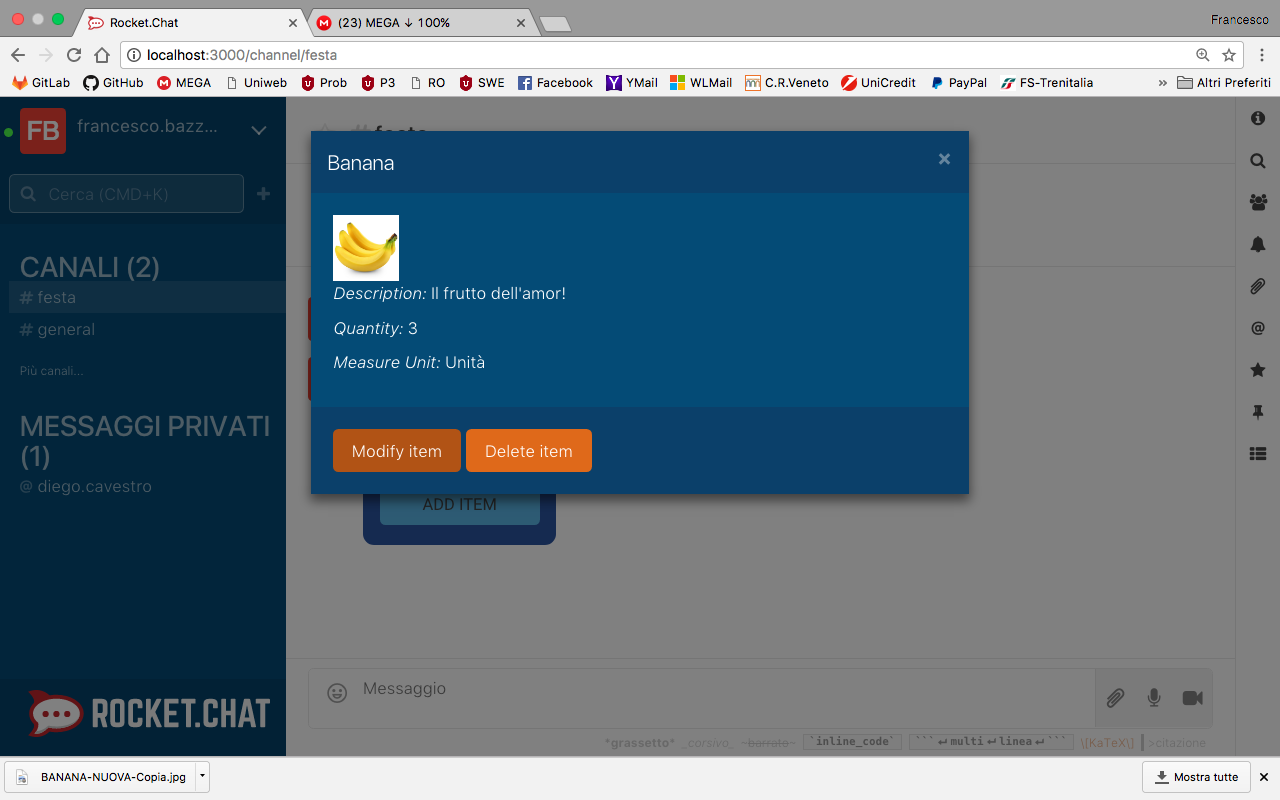
\includegraphics[width=\textwidth]{Sections/3-HowToUse/Images/item_details.png}
  \caption{Popup showing the item's information.}
\end{figure}

Now, click on the \textit{"Modify"} item, opening up the view to edit the item's data.

\begin{figure}[H]
  \centering 
  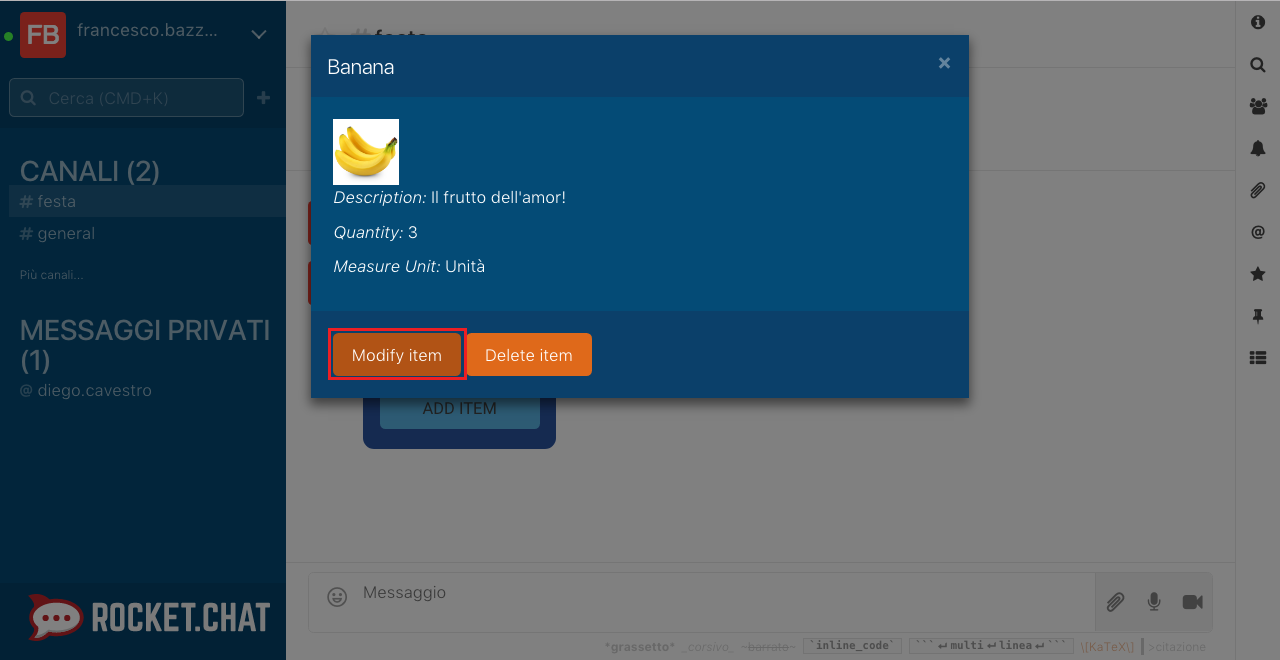
\includegraphics[width=\textwidth]{Sections/3-HowToUse/Images/popup_item_edit.png}
  \caption{View to edit the information about an item.}
\end{figure}

\begin{figure}[H]
  \centering 
  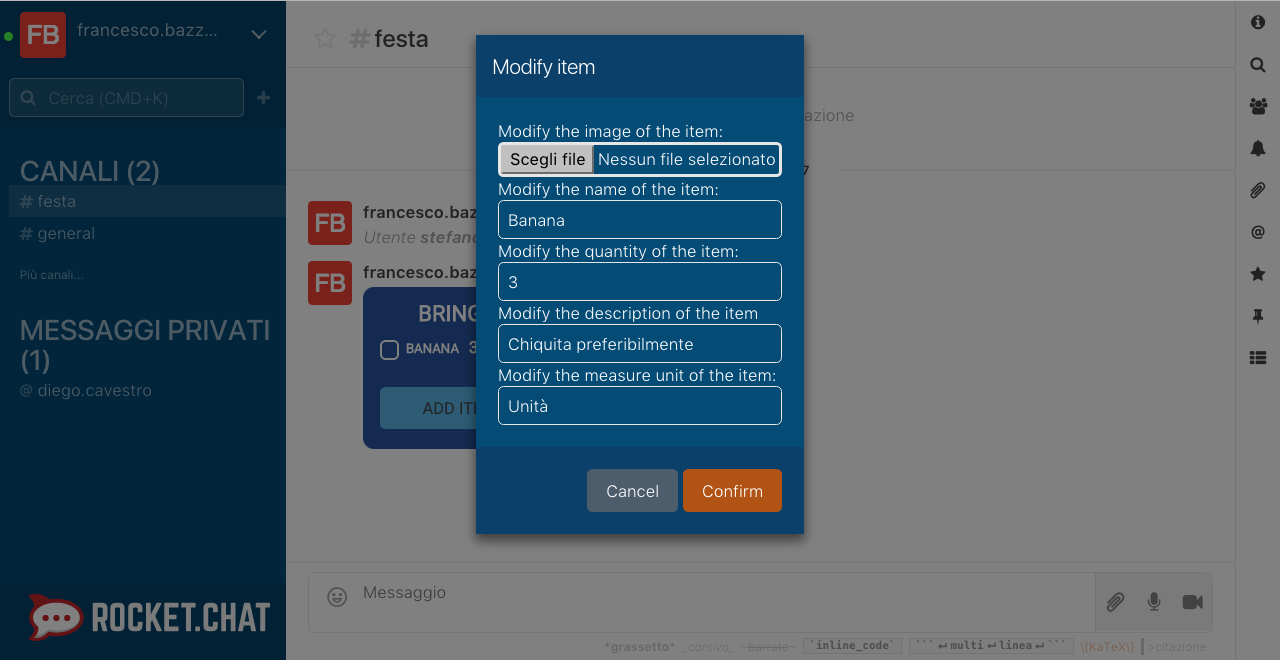
\includegraphics[width=\textwidth]{Sections/3-HowToUse/Images/popup_item_edit_filled.png}
  \caption{View to input the new information about an item.}
\end{figure}


Once you have modified all the information that you want, just click on the \textit{"Confirm"} button, which will save the edits you have performed.

% Immagine della bolla con l'oggetto modificato
\begin{figure}[H]
  \centering 
  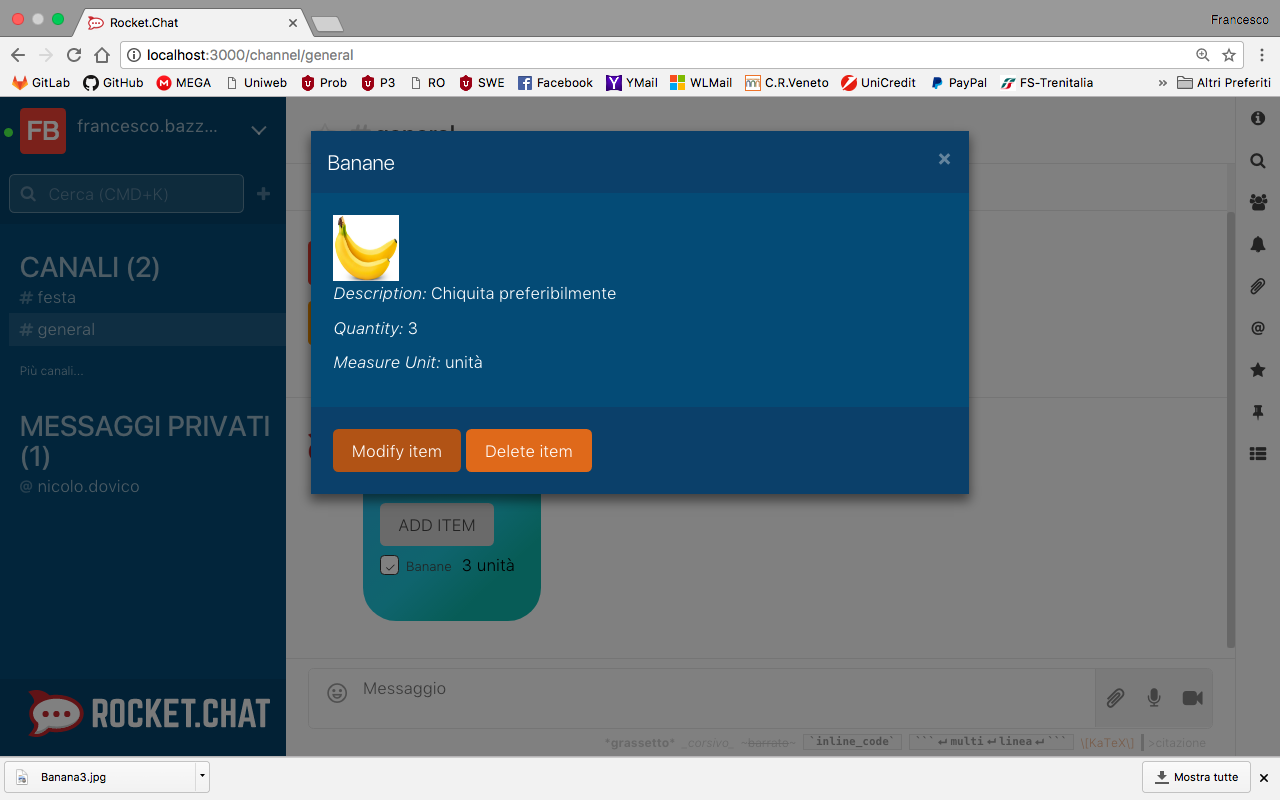
\includegraphics[width=\textwidth]{Sections/3-HowToUse/Images/item_edited.png}
  \caption{Popup showing the information of and edited item.}
\end{figure}